\newcommand{\ldshort}[1]{{\bf{[#1]}}\todo{define abbr #1}}
\newcommand{\lcite}[1]{\cite{#1}}
\newcommand{\ignore}[1]

\newduneabbrev{lsst}{LSST}{Large Synoptic Survey Telescope}{8.4 m telescope with 3.2G-pixel camera that will start taking data in 2023.}
\newduneabbrev{ska}{SKA}{Square Kilometer Array}{International radio telescope array planned to start data-taking in 2027.}
\newduneabbrev{hyperk}{HyperK}{Hyper Kamiokande}{260 kT water Cerenkov neutrino detector to begin construction at Kamiokande in 2020.}
% June 17, 2019 - recovered from github 

\chapter{Computing in DUNE}
\label{ch:exec-comp}

%%%%%%%%%%%%%%%%%%%%%%%%%%%%%%%%%%%%%%%%
\section{Executive Summary}
\label{ch:exec-comp-es}

The \dword{dune}  collaboration comprises 178 institutions from 32 countries, including 15 European nations and \dword{cern}. The experiment is preparing to commission the first 10kT  fiducial mass \dword{lar} \dword{tpc} module between 2024 and 2026 with a long data taking run growing to four modules between 2026 and 2036 and beyond.  An active prototyping program is already in place and has had  a short test beam run in 2018 at \dword{cern}.  These tests used  a 700T, 15,360 channel prototype \dword{tpc} with \dword{sp} readout.  Tests of a \dword{dp} detector of similar size are scheduled for mid-2019.   The \dword{dune} experiment has already  benefited greatly from these initial tests.  The collaboration has recently formed a formal \dword{csc}, with significant participation by European institutions and interest from groups in Asia, to develop common software and computing and to formalize resource contributions.

The consortium resource model benefits from existing \dword{osg}  and \dword{wlcg} infrastructure developed for the \dword{lhc} and broader \dword{hep} community.  \dword{dune}, through  \dword{pdsp}, is already using global resources for simulating and analyzing  \dword{pdsp} data.  Several European institutions are part of this resource pool and are making significant contributions to the \dword{pdsp} and \dword{pddp} programs.  We expect this global computing consortium to grow and evolve as we move towards gathering data from the full \dword{dune} detectors in the 2020s.

The \dword{dune} science program should produce raw data volumes similar in scale to the data volumes that current \dword{lhc} Run-2 experiments have already recorded.  Baseline predictions for the \dword{dune} data, depending on actual detector performance and noise levels, are $\ge 30$ PB of raw data per year.  These data, with simulations and derived analysis samples, must be available to all collaborating institutions.  We anticipate that institutions worldwide will be both contributors and end-users of storage and CPU resources for \dword{dune}.

To enable these resource contributions in cooperation with the \dword{lhc} and other communities, we plan to use common computing layers for infrastructure access and common tools to ease integration of facilities with both the \dword{dune} and \dword{lhc} computing ecosystems.  We will use common data storage methodologies to establish large high-availability data lakes worldwide  and to collaborate with the broader HEP community in developing other common tools.


HEP has considerable infrastructure in place for international computing collaboration thanks to the \dword{lhc} program.  Additional large non-\dword{lhc} experiments, including the \dword{lsst}, \dword{ska}, \dword{dune}, and \dword{hyperk},  will enter operation over the next decade and must use and expand upon this model for international cooperation.  Organizing the broader HEP community is formalized through the \dword{hsf} \cite{Alves:2017she}.  The \dword{hsf} is an organization of interested parties working to use the extensive knowledge gained over the past two decades and anticipate the needs experiments will have over the next two decades to develop a sustainable computing landscape for the HEP community.  The \dword{hsf} white papers and roadmaps emphasize common tools and infrastructure as the underpinnings of this landscape.

\dword{dune}'s computing strategy heavily leverages this model of common tools and infrastructure and features data movement and storage, job control and monitoring, accounting, and authentication that both use and contribute to this global community.   \dword{dune} recognizes that other large-scale experiments have similar needs and will encounter similar issues, thus driving worldwide cooperation on common tools as the most cost-effective way to fulfill the scientific missions of the experiments.  Already in the R\&D phases of \dword{dune} computing, \dword{dune} pilot programs use this model.  Most recently in data management and storage, \dword{fermilab}, \dword{cern}, Rutherford Appleton Laboratory, and other academic institutions in the United Kingdom are collaborating on adapting and using the \dword{rucio} data management systems \cite{Barisits:2019fyl}  to serve as the core data management system for \dword{dune}.

Examples of this proto-culture of international collaboration within \dword{dune} were demonstrated during the 2018 test beam run of the \dword{pdsp} detector.  The \dword{protodune} run was a valuable live test of this model.  During this run, the \dword{sp} detector at \dword{cern} produced raw data at rates exceeding 2GB/s.  These data were transferred and stored in the archive facilities at \dword{cern} and \dword{fermilab} and replicated at sites in the United Kingdom and Czech Republic.

In total, \SI{1.8}{PB} of raw data were produced during the 10 week test beam run, mimicking, within a factor of two, expected data rates and volumes from the initial running of the \dword{fd} complex .  The prototype run was used to examine and test the scalability of existing and proposed computing infrastructure and to establish operational experience within the institutions which have expressed interest in the development and construction of the \dword{dune} computing environment.  The technical design presented here builds heavily on the measurements and information gained from the \dword{protodune} experience.   These measurements are proofs of concept for many of the systems, and their behavior can be extrapolated to the projected levels needed for the full \dword{dune} experiment. 

In addition to traditional HEP computational strategies that have been prototyped in \dword{protodune}, the format and organization of \dword{dune}'s data as large multi-dimensional arrays open the possibility of treating the data with computing paradigms similar to those developed for astrophysical image data.  These image processing techniques heavily leverage advances in machine learning and pattern recognition.  Moreover, these techniques benefit from computing resources available at high performance computing (HPC) facilities (supercomputers), where massively parallel and computation heavy algorithms can be mapped onto hardware topologies where they scale better than with traditional batch farms.  Machine learning and HPC oriented analysis is a very active field with continuous advances coming from the current generation of \dword{lar} experiments such as \dword{argoneut}, \dword{microboone}, \dword{sbnd}, and \dword{icarus}.  \dword{dune} is poised to benefit from this work and to expand on it as part of its computing and analysis model.

In summary, \dword{dune}'s computing strategy must be global, working with partners worldwide, and collaborative because almost all computational challenges we face are also those facing similar experiments. 
 
%%%%%%%%%%%%%%%%%%%%%%%%%%%%%%%%%%%%%%%%
\section{Overview}
\label{ch:exec-comp-ovr}
The mission of the computing consortium is to facilitate the acquisition, processing, and analysis of both detector data and supporting simulations for the \dword{dune} experiment.  This mission must extend over all of primary physics drivers for the experiment and must do so both cost effectively and securely. The \dword{csc} provides the bridge between several online \dword{daq} and monitoring systems and the different physics groups who develop high-level algorithms and analysis techniques to perform measurements with the \dword{dune} data and simulation. The \dword{csc} works with collaborating institutions to identify and provide computational and storage resources.  They provide the software and computing infrastructure in the form of analysis frameworks, data catalogs, data transport systems, database infrastructure, code distribution mechanisms, and other support services essential for recording and analyzing the data and simulations. 

The \dword{csc} works with national agencies and major laboratories to negotiate use and allocation of computing resources.  This work includes support for near term and R\&D efforts like \dword{protodune} runs and extends to the design, development, and deployment of the \dword{dune} computing model and its requisite systems.
These designs include evaluating major software infrastructure systems, among them, workload management and data management systems, to determine their suitability for satisfying the \dword{dune} physics requirements.   These evaluations should identify opportunities to adopt or adapt existing technologies and engage in collaborative ventures with HEP experiments outside of \dword{dune}. 

In this context, the \dword{dune} computing needs are modest considering the projected rates and needs for the high luminosity \dword{lhc} experiments.  Initial calculations and extrapolations place the data volumes for the \dword{dune} \dword{fd} program on par with the volumes produced during \dword{lhc} Run-2.  On the other hand, the  beam structure, event sizes, and analysis methodologies make \dword{dune} very unlike collider experiments in event processing needs and projected computational budgets.  In addition, the large \dword{dune} event sizes present a novel technical challenge when data processing and analysis are mapped onto  current and planned computing facilities.  Neutrino oscillation analysis and parameter extraction also present novel computational challenges.   Some of these challenges may require significant effort to adapt to the global computing resources available to the experiment.  These global resources are likely both heterogeneous in computational capabilities (featuring CPU, GPU, and other advanced technologies) and diverse in topological architectures and provisioning models.  The \dword{dune} computing consortium must address these issues of diversity and architecture to fully exploit the global resources available after 2026 and enable all collaborators to access the data and perform the scientific mission of the experiment.  


\section{Consortium Organization}



%%%%%%%%%%%%%%%%%%%%%%%%%%%%%%%%%%%%%%%%
\subsection{Resources and Governance}
\label{ch:exec-comp-gov}

The computing and software group is now a \dword{dune} consortium.  Reference~\cite{bib:docdb12751} describes the governance structure for the consortium.  The consortium coordinates effort across the collaboration, but funding comes from collaborating institutions, laboratories, and national funding agencies. Aside from a small fraction of the consortium leadership \dword{fte}, it is not supported by DUNE or LBNF project funds.  

The consortium has an overall consortium leader. The consortium leader is responsible for the sub-system deliverables and represents the consortium in the overall \dword{dune} collaboration.

In addition, technical leads act as overall project managers for the consortium. The technical leads report to the overall consortium leader.
\dword{csc} has both a host laboratory technical project lead to coordinate between the \dword{dune} project and host laboratory and an external technical lead to coordinate with other entities.
At least one of the three leadership roles should be held by a non-US scientist. 
As with other \dword{dune} consortia, the \dword{csc} provisionally divides institutional
responsibilities for computing resources, deliverables, and operations among the participating institutions. This division of responsibilities must account for the resources that are likely to be available. The internally agreed upon division of responsibilities must be presented to the technical board, which will then recommend the collaboration management for approval.

\todo{Insert Org Chart}

\subsection{Scope of the Consortium}
The \dword{csc} focuses mainly on the infrastructure and resources for offline computing.  Responsibility for algorithm development resides within the physics groups while online systems at experimental sites are governed by the \dword{daq} and \dword{cisc} consortia. These groups coordinate closely to ensure that the full chain of data acquisition, processing, and analysis works. Formal interfaces with these groups are described in Docdb 7123 (DAQ)\cite{bib:docdb7123} and Docdb 7126 (CISC)\cite{bib:docdb7126}.

The \dword{csc} operates at two levels: at the hardware level, where generic resources can be provided as in-kind contributions to the collaboration, and at the human level, where individuals and groups help develop common software infrastructure. 

Thanks to the substantial investment in grid computing infrastructure and storage systems at major laboratories, CPU and long-term storage resources sufficient for development and protoDUNE reconstruction and analysis have come together very well.  However human resources dedicated to DUNE specific projects are still in the formative stages with very little funding as yet identified for full-time personnel. 

\begin{figure}[htp]
\centering
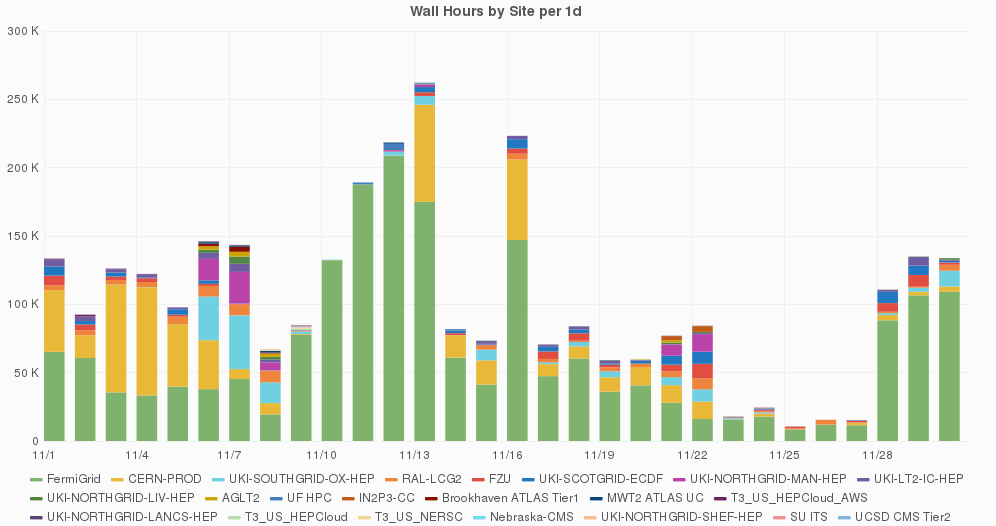
\includegraphics[height=4in]{graphics/comp-vo-summary.png}

\caption{CPU wall-time for November 2018 during ProtoDUNE-SP reconstruction showing multiple site contributions.  The major contributions were from FNAL, CERN, many UK institutions and FZU in the Czech Republic.}
\label{fig:ch-exec-comp-cpupie}
\end{figure}


\subsection{General Infrastructure}
As illustrated in Figure \ref{fig:ch-exec-comp-cpupie} the collaboration has already used substantial global resources through the \dword{wlcg} and \dword{osg} mechanisms. As the \dword{csc} evolves, institutions and collaborating nations will be asked to formally pledge resources (both CPU and storage), and those resources will be accounted for and considered in-kind contributions to the collaboration.
As illustrated above, several international partners are already contributing substantially. We are integrating additional large national facilities. Most resources are opportunistic, but \dword{fermilab} and \dword{cern} have committed several thousand cores and several PB of disk while \dword{dune} has been one of the first beneficiaries of the United Kingdom's IRIS project to provide computing for astronomy and particle physics.


\begin{dunetable}
[DUNE CSC members as of February 2019]{lll}{tab:exec-comp-consortium}{DUNE Computing and Software Consortium members as of February 2019, -- indicates sites not yet integrated into production computing. }%\rowtitlestyle
Institution& Country \\\colhline%& Integrated\\
KISTI&Korea\\\colhline %&--\\
TIFR  & India \\\colhline%& in process \\
Nikhef&NL\\\colhline%&Yes\\
Edinburgh&UK\\\colhline%&Yes\\
Manchester&UK\\\colhline%&Yes\\
RAL/STFC&UK\\\colhline%&Yes\\
Argonne&USA\\\colhline%&--\\
BNL&USA\\\colhline%&Yes\\
Cincinnati&USA\\\colhline%& Yes\\
Colorado State&USA\\\colhline%& Yes\\
CU Boulder&USA\\\colhline%&Yes\\
Fermilab&USA\\\colhline%& Yes \\
Florida &USA\\\colhline%& Yes\\
LBNL&USA\\\colhline%&Yes\\
Minnesota&USA\\\colhline%&Yes\\
Northern Illinois Univ.\\\colhline%&USA& --\\
Notre Dame&USA\\\colhline%&Yes\\
Oregon State University&USA\\\colhline%&Yes\\
Tennessee&USA\\\colhline%&--\\
Texas, Austin&USA\\%&--\\
\end{dunetable}

\subsection{People}

The \dword{csc} has (or will have) subgroups for the following areas.  Highlights of some of the ongoing projects are detailed in subsequent sections. 

\begin{itemize}
    \item collaborative tools,
\item data storage and management,
\item databases,
\item production and processing, 
\item workflow management,
\item \dword{dqm},
\item software release management, 
\item core software (led by a software architect),
\item advanced architectures,
\item algorithm liaisons, and 
\item networking.
\end{itemize}

\subsection{Work packages}
The definitions of work packages and assignment to institutions is still being developed. Different institutions have different competencies and it is important to understand what needs to be done before deciding who will do it.  The \dword{csc} is instituting a series of workshops, starting with Data Model and Infrastructure in the summer of 2019, to understand the scope of subprojects in preparation for a formal TDR. 

\section{Data Types and Volumes}

%The DUNE data structure is considerably different from previous neutrino and present collider experiments. Neutrino experiments, including DUNE, run at low rates - of order 1 Hz even for near detectors. But DUNE, due to the large volume and number of channels can generate enormous amounts of data from a single readout.
%This leads to unique new challenges in data storage and reconstruction, even where the data volumes and CPU needs are significantly smaller than those for large collider experiments.  In this section we describe the data volumes and types expected for normal running, calibration and supernova readouts of the far detector. 

% text recovered from the iDR

Offline computing for  \dword{dune} faces new and considerable challenges due to the large scale and diverse physics goals of the experiment.  In particular, the advent of \dword{lar} TPC's with exquisite resolution and sensitivity, combined with enormous physical volumes, creates challenges in acquiring and storing large data volumes and in analyzing and reducing them.  
As a result, the DUNE data structure is considerably different from previous neutrino and present collider experiments. Neutrino experiments, including DUNE, run at low rates - of order 1 Hz even for near detectors. But DUNE, due to the large volume and number of channels can generate enormous amounts of data from a single readout.
This leads to unique new challenges in data storage and reconstruction, even where the total data volumes and CPU needs are significantly smaller than those for large collider experiments.  

The computing landscape is changing rapidly, with the traditional HEP architecture of individual cores running single-threaded applications being superseded by applications efficiently utilizing multiple processors and perhaps demanding GPUs. At the same time, algorithms for \dword{lar} reconstruction are still in their infancy and developing rapidly.  As a result, we have reason to be optimistic about the future but we are not able to predict it accurately.  The \dword{protodune} single test at CERN in the fall of 2018 has provided a wealth of data that will inform the future evolution of  the \dword{dune} computing models.

In this section we describe the data volumes and types expected for normal running, calibration and supernova readouts of the far detector and the potential for the near detector. 



\subsection{Detectors}

The  \dword{dune} offline computing challenges can be classified in several ways.  We will start with the different detector/physics configurations that drive the large scale data storage and reconstruction. 
%This discussion leans heavily on the \dword{daq} design described in \voltitlespfd and \voltitledpfd  of the \dword{dune} Technical Proposal

The \dword{dune} experiment will consist of four 10~kT fiducial mass far detector modules located at  the Sanford Underground Research Facility, using either single or dual phase Liquid Argon TPC's, and an, as yet unspecified, near detector at Fermilab.
The proposed  full-size  modules for the far detectors will  have an active volume 12m high, 14.5m wide and 58m long. 

\subsubsection{Single-phase technology data estimates}
 Each  \dword{sp}  module will consist of 
150 alternating vertical cathode and anode planes  spaced 3.5 m apart and operated at 180~kV for a 500~V/cm drift field.  The anode planes are made up of \dword{apa}s which are 6.3~m tall by 2.3~m wide and have 2,560 readout channels each. Each channel is sampled with 12-bit precision every 500 nsec. 
For modules of this size, drift times in the liquid argon are of order 2.5~ms and raw data sizes before compression are of order 6~GB per module per 5.4~ms readout window.  With no triggering and no zero suppression or compression, the raw data volume for four modules would be of order 145~exaB/year. Table \ref{tab:exec-comp-bigpicture} summarizes the relevant parameters for the \dword{sp} technology.


\begin{dunetable}[Useful quantities for computing estimates]{lrr}{tab:exec-comp-bigpicture}
{Useful quantities for computing estimates for single phase readout}%\rowtitlestyle
Quantity&Value&Explanation\\ 
\hline
{\bf Far Detector Beam:}\\ \colhline
Single APA readout &41.5 MB& Uncompressed 5.4 ms\\ \colhline
APAs per module& 150&\\
Full module readout &6.22  GB& Uncompressed 5.4 ms\\ \colhline
Beam rep. rate&\beamreprate&Untriggered\\ \colhline
CPU time/APA&100-200 sec&from MC/ProtoDUNE\\ \colhline
Memory footprint/APA&2 GB&ProtoDUNE experience\\ \colhline
{\bf Supernova:}\\ \colhline
Single channel readout &270 MB& Uncompressed 90 s\\ \colhline
Four module readout& 600 TB& Uncompressed 100 s\\ \colhline
Trigger rate&1  per month&(assumption)\\

\end{dunetable}


\begin{dunefigure}[Figure from volume \todo{pointer to SP DAQ section} Expected physics-related activity
    rates in one FD module]{fig:daq-rates}{Expected physics-related activity
    rates in a single \nominalmodsize module. \label{sec:fd-daq:rates}
}
  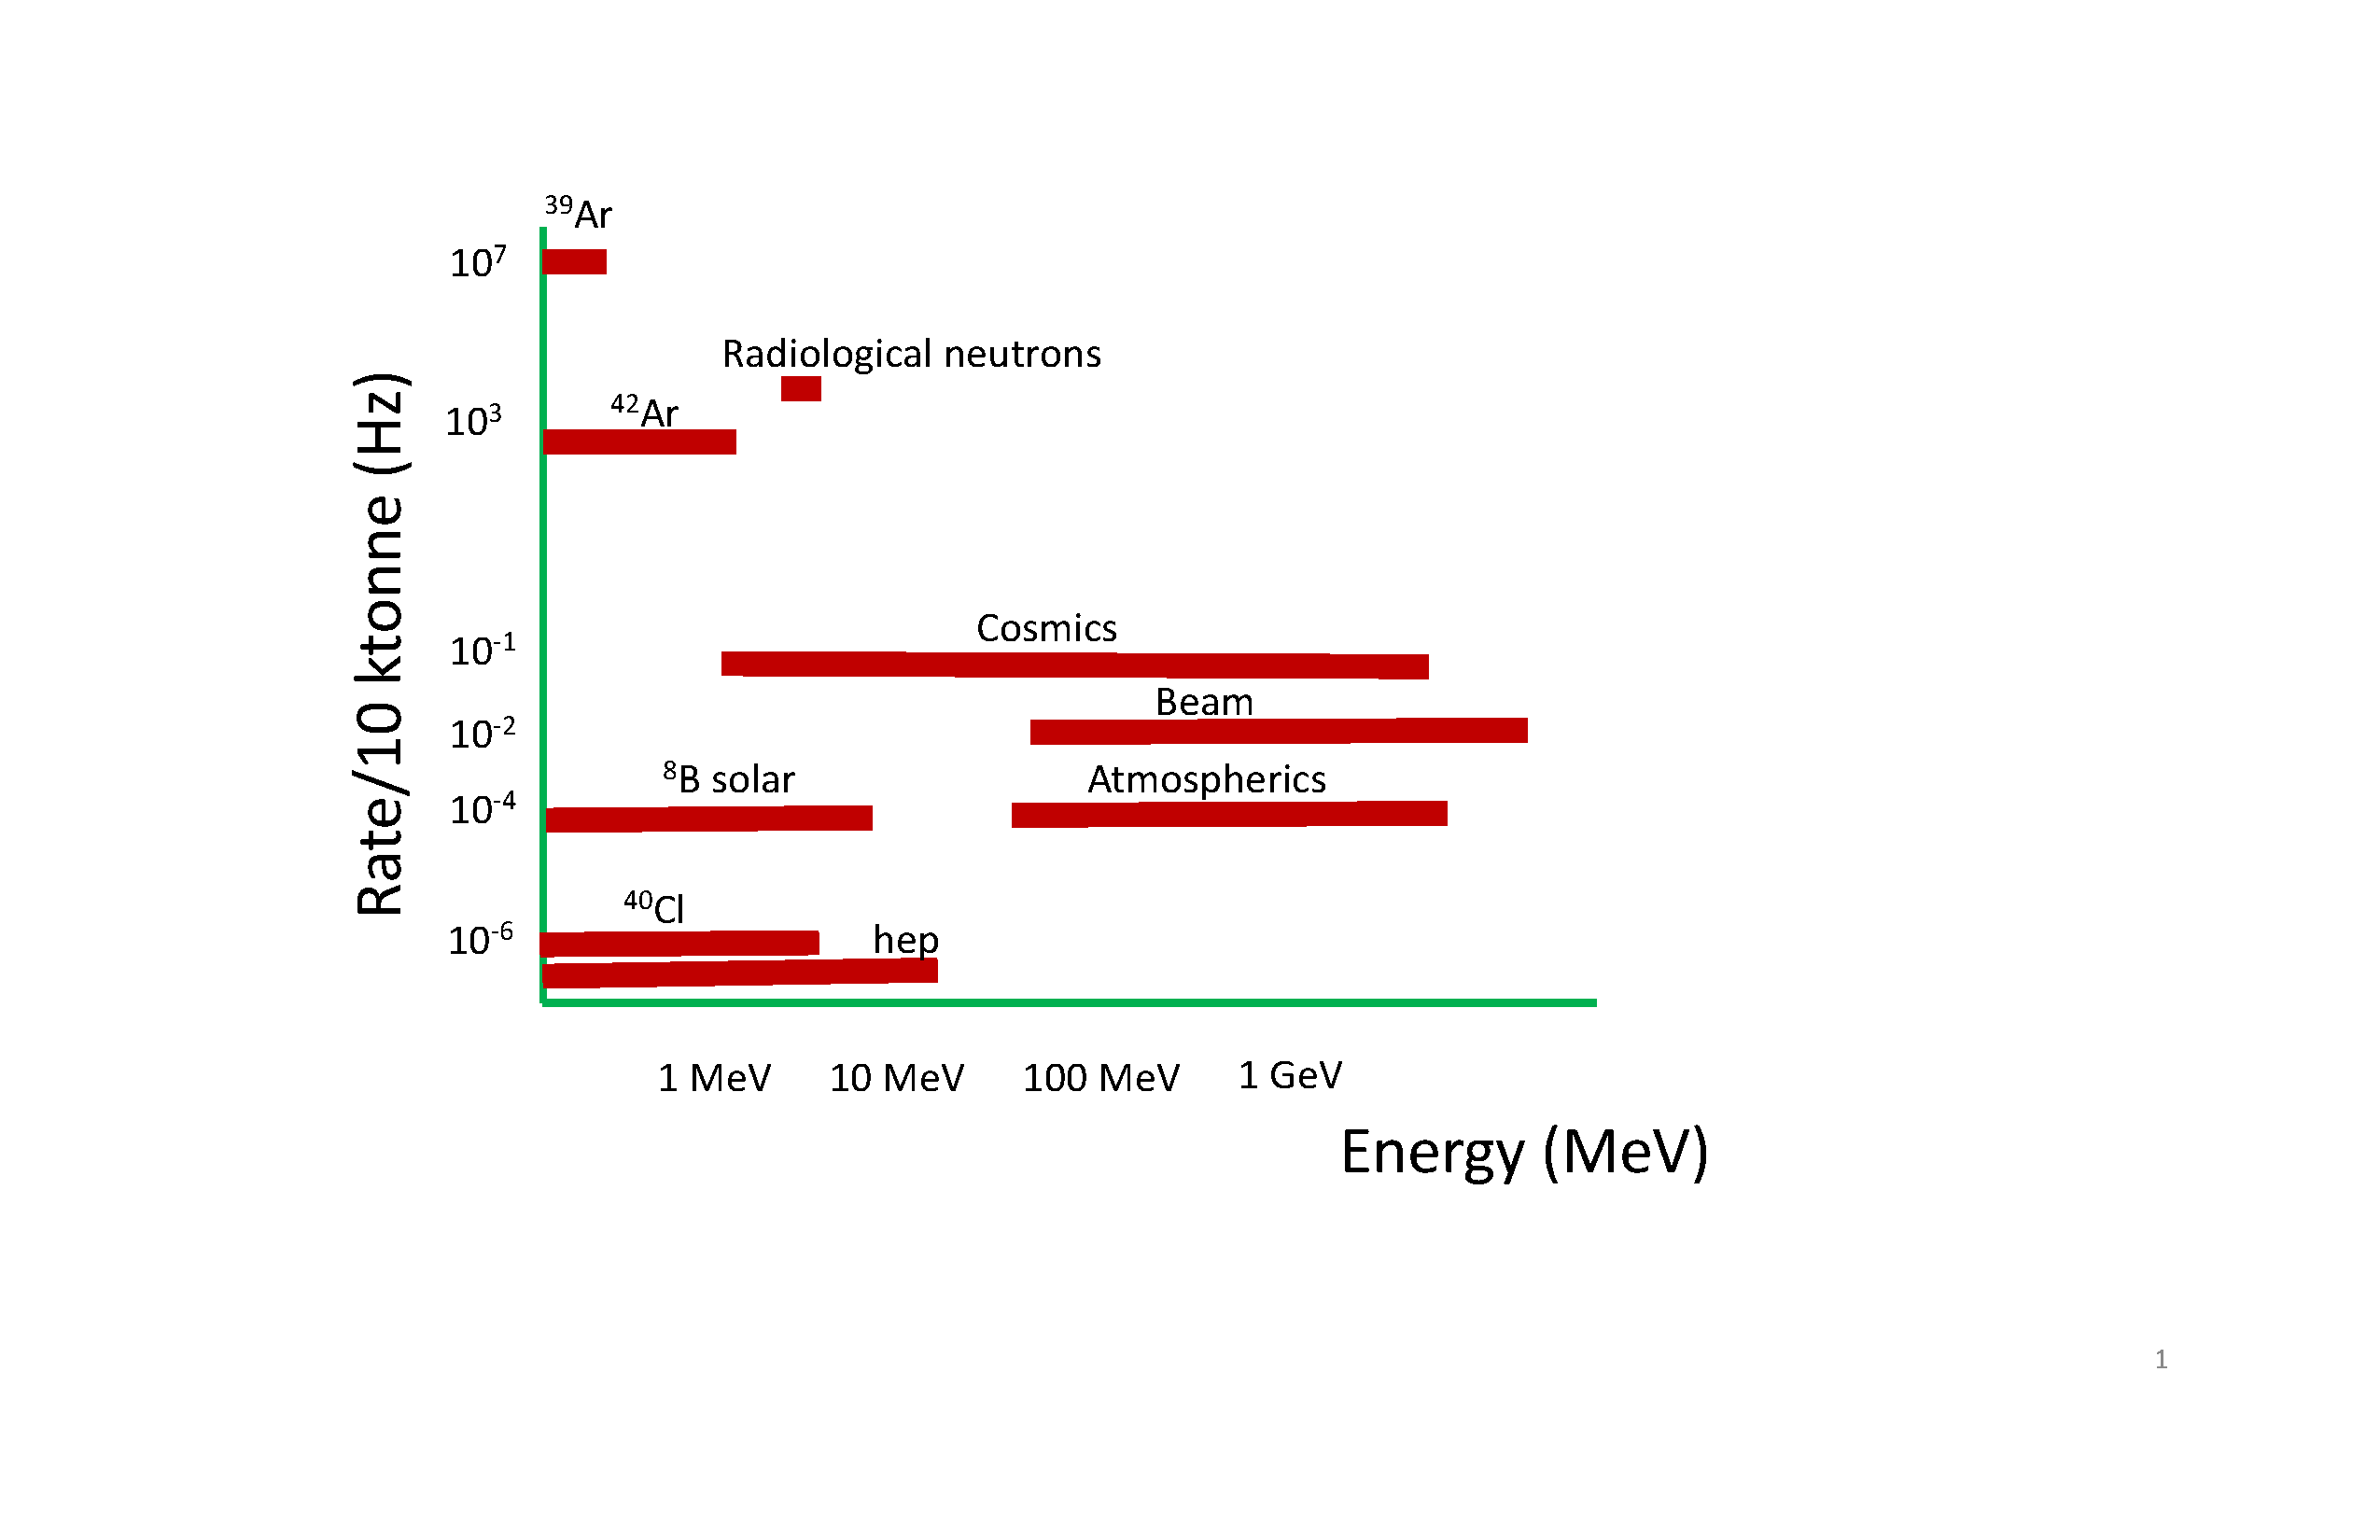
\includegraphics[width=0.7\textwidth,clip,trim=6cm 6cm 10cm 2cm]{daq-event-type-rates-vs-energy.pdf}
\end{dunefigure}

\begin{dunetable}
[Expected DAQ Yearly Data Rates]
{p{0.3\textwidth}p{0.1\textwidth}p{0.5\textwidth}}
{tab:daq-data-rates-sp}
{Summary of expected data rates for initial single-module running with single-phase technology from Volume XXX. The rates assume no compression, and are given for a single \SI{10}{\kilo\tonne} module. Trigger primitives are not kept permanently; they are temporarily stored for 1-2 months at a time. The same applies to fake \dword{snb} data. Improved readout algorithms will be developed and evaluated with the initial data and are expected to provide about an order of magnitude reduction in data while retaining efficiency.}
Source  & Annual Data Volume & Assumptions \\ \toprowrule
Beam interactions & 27 TB & 10 MeV threshold in coincidence with beam
time, including cosmic coincidence; \SI{5.4}{\milli\second} readout \\ \colhline
Cosmics and atmospheric neutrinos & 10 PB & \SI{5.4}{\milli\second} readout \\ \colhline
Radiological backgrounds & $<2$ PB & $<1$ per month fake rate for SNB
trigger\\\colhline
Cold electronics calibration & 200 TB & \\ \colhline
Radioactive source calibration & 100 TB & $<10$ Hz source rate; single
APA readout; \SI{5.4}{\milli\second} readout \\\colhline
Laser calibration & 200 TB & 10$^6$ total laser pulses; half the
TPC channels illuminated per pulse; lossy
compression (zero-suppression) on all channels\\\colhline
Random triggers & 60 TB & 45 per day\\\colhline
Trigger primitives & 13 PB & Dominated by $^{39}$Ar (50~kHz per APA face); collection
channels only; 20 bytes per trigger primitive \\\colhline
\end{dunetable}



\subsubsection{Dual-phase technology}

For dual-phase, electrons drift the full height of the cryostat, emerge from the liquid and are collected - after gas amplification, on an grid of instrumented pads at the top of the detector.  The WA105 3x1x1 m test of this technology ran successfully in the summer of 2017\cite{Murphy:20170516}. 
Each 17~kT module will have 153,600 channels. Drift time in the liquid argon is 7.5 ms. Given 20,000 samples in an 8~ms readout, the uncompressed event size is 4.2~GB (for 1 drift window).  Due to gas amplification, the signal to noise ratio is quite high, allowing loss-less compression to be applied at the front-end  with a compression factor of ten, bringing the event size/module to 0.42~GB. Recording the entire module drift window can be considered a pessimistic figure, since events are normally contained in smaller detector regions. A  far detector module can be treated as 20 smaller  detectors (with similar number  of readout channels to the prototype currently being constructed at CERN), running in parallel, each one defining a Region of Interest  (\dword{roi}). For beam or cosmic events it is possible to record only the interesting ROI(s) with the compressed size of a single ROI being 22~MB.

\subsection{Data rates}
\subsubsection{Beam coincident rates}

Requiring  coincidence with the \dword{lbnf} beam will reduce the effective live-time from $1/$\beamreprate  to a 5.4~ms (8~ms for DP)  readout window coincident with the 10 microsecond beam spill, leading to an uncompressed data size for beam-coincident events of around 24 GB for four 17~kT single-phase detector modules (and somewhat less for dual-phase), too high to record permanently at full rate.
Only a few thousand true beam interactions in the far detectors are expected each year.  Compression and conservative triggering based on photon detectors and ionization should reduce the data rate from beam interactions by several orders of magnitude without sacrificing efficiency.  Studies discussed in the \dword{daq} section of this proposal indicate that high efficiencies are achievable at an energy threshold of 10 MeV, leading to event rates for beam-initiated  interactions of $\sim 6,400$/year.

\subsubsection{ Near detector} The near detector configuration is not yet fully defined  but we do have substantial experience from T2K and  \dword{microboone} at lower energies, and  \dword{minerva} at the  \dword{dune} beam energies on cosmic and beam interactions under similar conditions.  We can expect that a near detector will experience $\sim$ 5-10 beam interactions/beam pulse and non-negligible rates of cosmic rays, spread over an area of a few square meters. \dword{microboone} experience and \dword{protodune} simulations indicate compressed event sizes of 100-1000 MB, leading to yearly data volumes of 2-20 PB.  Storing and disentangling this information will be challenging but comparable to the \dword{protodune} data already recorded. 








\subsubsection{Processes not in synchronization with the beam spill} These include supernova physics, atmospheric neutrinos, proton decay, neutron conversion and solar neutrinos.  These processes are generally at lower energy, making triggering more difficult, and asynchronous, thus requiring an internal or external trigger.  In particular, supernovae signals will consist of a large number of low-energy interactions spread throughout the far detector volume over a time period of 1-100 seconds. Buffering and storing 100 seconds of data would require around 20,000 readout windows, or around 600~TB per 4-module supernova readout.  At a rate of one fake \dword{snb} event/month, this is around 7~PB of uncompressed data per year. 

\subsubsection{
Calibration}
In addition to physics channels, continuous calibration of the detectors will be necessary.  It is likely that, for the far detectors, calibration samples will  dominate the data volume. Cosmic-ray muons and atmospheric neutrino interactions will provide a substantial sample for energy and position calibration.  Dedicated runs with radioactive sources and laser calibration will also generate substantial and extremely valuable samples. Table \ref{tab:daq-data-rates-sp} includes estimates for the single-phase far detector.   Cosmic ray and atmospheric neutrino signals collected for calibration make up the bulk of the uncompressed \dword{sp} data volume at $\sim$ 10~PB/year per 17~kT module and will dominate the rates from the far detectors.  













\subsubsection{Zero suppression}

The data volumes discussed above are for un-zero-suppressed readout of the full detector. A combination of local triggering, zero-suppression and  efficient lossless compression mechanisms can substantially reduce the final data volume but previous experience in HEP indicates that signal processing must be done carefully and often happens well into data-taking when the data are well understood.  Experience from  \dword{microboone} and the \dword{protodune} experiments will aid us in developing these algorithms but it is likely that they will be applied later in the processing chain for single-phase.  No zero-suppression is planned for dual-phase.

The constrained environment at the Sanford Lab motivates a model where any further data reduction via zero-suppression is done downstream, either on the surface or after delivery to computing facilities at FNAL or elsewhere. This could be analogous to the HLT's used by LHC experiments. The relative optimization of data movement and processing location is an important consideration for the design of both the \dword{daq} and offline computing.

\subsection{Data storage and retention policies}
Some of the samples listed above are extremely valuable and will require conservative retention policies.  Examples include real neutrino and cosmic ray interactions in the far detector, most of the near detector data and any real supernova events. Calibration samples and, potentially, fake \dword{snb} triggers may be stored temporarily and discarded after processing. 

\subsection{Summary}
In summary, uncompressed data volumes will be dominated by calibration for the far detectors 10-15 PB/year/module and by beam and cosmic ray interactions in the near detectors.  With four \dword{fd} modules but a conservative factor of four for lossless compression a total compressed data volume of 10-15~PB/year for the far detectors is anticipated. Near detector rates are not known but likely to be similar.

After discussion with the \dword{sp} Trigger/\dword{daq} group, we asked them to include as upper limits in their design a  maximum data transfer rate from the far detectors to Fermilab of \surffnalbw, which is consistent with projected network bandwidths in the mid 2020's and a limit of 30~PB/year raw data stored to tape.  
%Table \ref{daq:datarates} summarizes the data rates expected from the \dword{daq} section of this proposal. 



\ignore{
\subsection{Basic readout parameters}

The maximum data rate that the \dword{dune} \dword{fd} modules can produce for a single readout is computed from the detector channel counts, base sampling rates, and digitization resolution.  This is then scaled by the expected triggering rates for beam induced activity along with other sources of trigger initiation (e.g., cosmic ray activity, radiological signals, calibration information) to compute the expected upper limit on the data rates and volumes that can be expected from the detector.  Separate estimates of the effects of lossless data compression and zero suppression schemes are estimated and, in some cases, demonstrated with the \dword{protodune} \dword{sp} data.  These techniques depend highly on the structure of the data and, in particular, the structure of the noise or other sources of background observed in the final \dword{dune} detector modules.  As a result, the compression/suppression estimates are given as ranges using detector performance assumptions.

The parameters described in Table~\ref{tab:exec-comp-bigpicture} display the key characteristics of the \dword{dune} \dword{fd} data stream.  A bandwidth specification provides an operational envelope within which the data acquisition, networking, and software and computing tasks should  operate. This bandwidth envelope has been set to  30~PB of data/yr.  This corresponds to a time-averaged egress bandwidth  of 950 MB/s (7.6 Gbit/s).  As an uncompressed event stream, this equals 0.15 evt/s, rising to 0.6 evt/s under a target compression of 4:1 of \dword{sp} module readout. Reducing the full streaming data rates to these rates should be implemented in the \dword{daq}/trigger level of the experiment. 
Those decisions are the purview of the collaboration scientists and the data acquisition design with feedback from \dword{csc} on what is possible.  The \dword{protodune} experience has provided invaluable feed back for the experiment design. 

\todo{The above text is redundant with the earlier explanations. need to merge and make consistent with DAQ section}
}
\ignore{
\subsection{Far Detector}

The computing model must be able to handle a wide range of data inputs from the \dwords{fd}, as documented in more detail in~\cite{bib:docdb9240}.

\begin{itemize}
\item Supernova triggers with an uncompressed size of 138 TB for a 30 second readout of all channels in a 4-module \dword{sp} detector at a likely rate of 1/month;  
\item Beam neutrino interactions within a single detector module with an uncompressed size of $\approx$ 6.2 GB.  Beam neutrinos arrive at a rate of up to 1 Hz, but most do not provide measurable interactions;
\item Atmospheric neutrino interactions, nucleon decay, and other lower energy processes confined to a subset of a detector module with a low threshold largely driven by radiological backgrounds;
\item Cosmic ray and rock muons at a rate of around 4,500/day/module; and
\item Other calibration systems.
\end{itemize}

The estimates in~\cite{bib:docdb9240}, with conservative estimates for increased needs for low level data taking during commissioning, have led to a negotiated upper limit of 30 PB/year data volume as a standard for both the trigger and data acquisition; the computing groups are working toward that goal. 
}


\ignore{
\subsection{Near Detector}
In addition, a \dword{nd} of reasonable size has multiple neutrino interactions/beam spill, which requires a read out at the full beam rate of 0.8-1.2 Hz.
The \dword{nd} has fewer channels and better signal/noise discrimination but much higher readout rates.  While the details of the detector design are still unknown, we assume data volumes of similar size to the far detector (30 PB/year) in our planning.
}

\subsection{Simulation}
The bulk of data collected with the \dword{fd} is likely to be background, with real beam interaction events in the \dword{fd} numbering in the thousands/year, not millions. Thus, the size of simulation samples may be less than the unprocessed raw data considered above.  Lower energy events are either very rare or can be simulated in sub-volumes of the whole detector.  As a result, while simulation will be important to the experiment, it should not dominate data volume as it does in many experiments.  

However, simulation inputs such as flux files, overlay samples, and shower libraries pose a special problem because they must be distributed to simulation jobs carefully.  Proper simulation requires that these inputs be distributed in unbiased parcels.  This can be technically difficult to do efficiently in a widely distributed environment and will require thoughtful design. 

\subsection{Analysis}

Analysis formats have not yet been fully defined.  We anticipate that most analysis samples will be many times smaller than the raw data.  However, because they are idiosyncratic to particular analyses and even users,  producing and cataloging them will be sociologically difficult. 
Likely we need a mix of official samples, produced by physics groups and distributed through a common catalog and file transfer mechanisms, as well as small user samples on local disks. 


\section{ProtoDUNE-SP as an Example}
\label{ch:exec-comp-proto-SP}
The first \dword{protodune} \dword{sp} run at \dword{cern} in late 2018 has already led to a small scale test of the global computing model.  In the following, we will describe the \dword{protodune} data design and the lessons learned from our experience. Much of this carries over into planning for full \dword{fd} operations. 

\subsection{Introduction}

The \dword{pdsp} detector ran at \dword{cern} in the NP04 beamline from September to November of 2018. Since then, studies of cosmic rays have continued. Before that run, several data challenges at high rate validated the data transfer mechanisms. 

\subsection{Data Challenges}

\dword{protodune} performed a series of data challenges, starting in late 2017.  Simulated data were passed through the full chain from the event builder machines to tape storage at \dword{cern} and \dword{fermilab} at rates up to 2 GB/s.  These studies allowed optimizing the network and storage elements well before the start of data taking.
Please note that the full \dword{dune} \dword{fd} would, in writing 30 PB/year, produce data at rates similar to or less than those demonstrated in the 2018 data challenges. 

\subsection{Commissioning and physics operations}

The first phase of operations was commissioning the detector readout systems while the \dword{lar} reached full purity.  Data were taken with cosmic rays and beam during the commissioning period. Once high \dword{lar} purity had been achieved, physics data were  taken with beam through October and half of November. Normal trigger rates were approximately 25 Hz, but tests were done at rates up to 100 Hz. Since the beam run ended, cosmic-ray data continues to be taken with varying detector conditions, such as modified high voltage and purity and new readout schemes. 

%\subsection{Data Quality Monitoring}

%\todo{DQM}

\subsection{Data Volumes}
The single-phase \dword{protodune} detector comprises a \dword{tpc} with  six \dword{apa}s, \dword{pd}s, and a \dword{crt}. In addition, the np04 beamline is instrumented with hodoscopes and Cerenkov counters to generate beam triggers. Random triggers  were generated at lower rates to collect unbiased cosmic ray information. The data volume from the test beam run was dominated by readout of the \dword{tpc}.  Each \dword{apa} has 2,560 channels and reads out 12 bit \dword{adc} values at 2 MHz.   The nominal readout window during beam running was  3 ms to match the drift time at the full voltage of 180 kV, which was maintained for most of the run.  The size of the \dword{tpc} data without compression was thus 138 MB/event, not including headers.  The uncompressed event size including all \dword{tpc} information and \dword{crt} and \dword{pd} data was 170-180 MB. Compression was implemented before the October beam physics run, reducing the total size per event from around 180 MB to 75 MB.  

\begin{dunetable}[Data volumes]{lrr}{tab:exec-comp-pd-volumes}{Data volumes  recorded by \dword{pdsp} as of December 2018.}
Type  & Events & Size\\ \rowtitlestyle
Raw Beam&8.08 M& 520 TB \\ \colhline
Raw Cosmics&3.46 M& 271 TB\\ \colhline
Commissioning&3.86 M& 388 TB\\ \colhline
Pre-commissioning&13.89 M&641 TB\\
\end{dunetable}

Events were written out in 8 GB raw data files with each containing approximately 100 events. The beam was live for two 4.5 s spills every 32 s beam cycle, and data were taken at  rates up to 50 Hz (typically 25 Hz) leading to compressed \dword{dc} rates of 400-800MB/sec from the detector.  Each beam cycle could, therefore, produce 1-4  8 GB output files.  In earlier runs with uncompressed data, and during an April data challenge, transfer rates up to 2GB/s were demonstrated over substantial periods. 

Beam was stopped on November 12, but detector cosmic ray studies continue, some with an increased time window of 7.5 ms to collect more complete tracks for each readout.  This raises the compressed event size to around 170 MB.


\subsection{ProtoDUNE-SP Data Streams}
The \dword{pdsp} data consist of multiple sources in addition to the \dword{tpc} data. One of the major challenges for offline computing systems is merging these data streams into a coherent whole for analysis.  Table \ref{tab:exec-comp-pd-sources} lists the data sources used and their granularity. 

\begin{dunetable}[Data sources]{lrr}{tab:exec-comp-pd-sources}{Data sources.  }
Type & indexed by & destination\\ \colhline
TPC  & run/event & event data\\ \colhline
Photon Detector data & run/event & event data\\ \colhline
Cosmic Ray Tagger & run/event & event data\\ \colhline
Beamline devices & timestamp & beam database\\ \colhline
Detector conditions & timestamp & slow controls database\\ \colhline
DAQ configuration & run & files/elisa logbook\\ \colhline
Run quality & run & human generated spreadsheets\\ \colhline
Data quality & run/event/time & Data Quality web application\\ \colhline
File metadata & file & sequential access via metadata file database\\
\end{dunetable}

Information about the detector conditions, \dword{daq} configuration, and run quality is spread across a number of sources and must be collected and then reduced to quantities relevant for offline data analysis.  For example, the \dword{sc} system logs detector conditions continually.  Offline analysis must know about data with coarser granularity and have algorithms that can use that information. A full conditions database transfer mechanism is being developed but was not available during the run.  As a result, other than beamline information, coarse information is currently added to the \dword{sam} file catalog run by run to allow files with given operating conditions to be easily identified and retrieved. Beam data is stored in the \dword{ifbeam}
database and connected to event data via time stamps.

\subsection{Reconstruction of ProtoDUNE-SP data}
Thanks to substantial previous effort by the \dword{35t} prototype, \dword{microboone} and the \dword{lar} \dword{tpc} community, high quality algorithms were already in place to reconstruct the \dword{tpc}  data.  As a result, a first pass reconstruction of the \dword{pdsp} data with beam triggers was completed by early December, less than a month after data taking ended.  Results from that reconstruction are presented in the Methods section of Volume~\volnumberphysics,\voltitlephysics{} with some highlights summarized here. 



\subsection{Data Preparation}

Before pattern recognition, data from the \dword{protodune} detector is
unpacked and copied to a standard format within the art framework based on ROOT \fixme{ROOT is in the common glossary but without a definition. I have not used the dword because I'm sure it's the same ROOT.} derived objects. 
The format is also used in detector simulation events.
This reformatted raw data includes the waveform for each channel, consisting of 6,000-15,000,  12-bit, 0.5 $\mu$sec samples. 

The first step in reconstruction is data preparation to
convert each \dword{adc} waveform into a calibrated charge waveform with
signals proportional to charge. At the end of data preparation, \dword{roi}s, i.e., blocks of contiguous samples where
useful signals appear, are identified, and the data outside these regions are discarded.



The sequence is described more fully in~\cite{bib:docdb12349} and in the Methods section of the Volume~\volnumberphysics,\voltitlephysics{}, but is summarized here: \fixme{get methods sec ref}

\begin{enumerate}
\item Each waveform is unpacked into integers.
\item Pedestals are determined per event/per channel from the most common \dword{adc} value. 
\item Pedestals and calibrations are applied. %\label{local:ped}
\item Bad channels, sticky bits, and other known hardware problems are corrected or removed.
\item Signal undershoot that creates a long negative tail is removed. 
\item The waveforms  are deconvoluted.  In the first processing, this was done with simple 1D  convolution for a single wire.  A \twod  method of deconvoluting a detailed detector electrostatic field map, originally developed for \dword{microboone}\cite{Adams:2018dra}, is  now available for \dword{protodune} and will be used in the future reconstruction passes.  It properly undoes the long-range induction effects while keeping efficiency high and bias low.  The deconvolution Fourier transforms the waveform, replaces the  bipolar field response function with a unipolar function, applies a low-pass filter to remove high-frequency noise, and then transforms back.

\fixme{One dimensional (1d) and two dimensional (\twod) should be consistent with one another and probably in LATEX code. (Anne says: I just use \twod and \threed from defs for consistency.)}




\item Finally, regions of interest are defined where the signal exceeds a given threshold, and time slices well outside the \dshort{roi} are dropped, significantly reducing the size of the remaining data. These data feed into the reconstruction algorithms for further pattern recognition. %\label{local:roi}
\end{enumerate}


Figures~\ref{fig:ch-exec-comp-chtraw} and~\ref{fig:ch-exec-comp-chtroi} illustrate the transformation of \dword{tpc} data  during data preparation.

\begin{figure}[t]
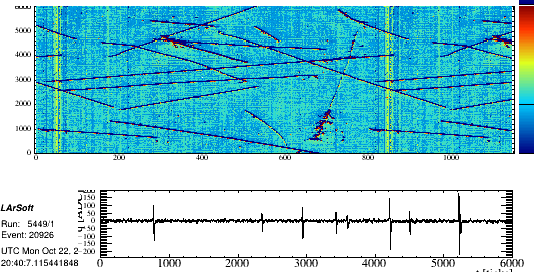
\includegraphics[width=\textwidth,angle=0]{comp-evd_twq-proj_5449_20926_raw.png}
\caption{Example of pedestal-subtracted data for one of the ProtoDUNE  wire planes.  The top pane shows the ADC values in a V (induction) plane with the x-axis being channel number and the y-axis, time slice. The bottom pane shows the bipolar pulses induced on one channel. 
}
\label{fig:ch-exec-comp-chtraw}
\end{figure}

\fixme{anne commented out includegraphics line because graphic not found - HMS - how did these get lost? THey were there in previous draft - I reloaded them}
\begin{figure}[t]
 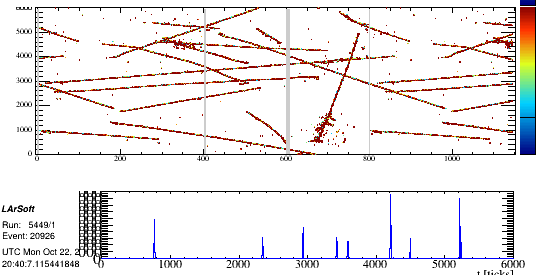
\includegraphics[width=\textwidth]{comp-evd_twq-proj_5449_20926_decon.png}
\caption{
Same as Figure~\ref{fig:ch-exec-comp-chtraw} except after calibration, cleanup, deconvolution and ROI finding. 
}
\label{fig:ch-exec-comp-chtroi}
\end{figure}
\fixme{anne commented out includegraphics line because graphic not found - it is there in github version}

\subsection{Computational Characteristics of Data Preparation and Deconvolution }
Decoding for \dword{pdsp} is currently done with all six \dword{apa}s in memory. Because each \SI{3}{ms} of \dword{apa} readout consists of more than \SI{15}{M} 16-bit values, decompressing and converting to floating point causes substantial memory expansion.  Decoding and deconvolution of six \dword{apa}s with 3 ms readout fits within a normal 2 GB memory/core footprint, but the 7.5 ms readout window used in some cosmic ray studies requires a correspondingly larger memory footprint. Because electrical signals are correlated between channels within an \dword{apa} wire plane but not between planes, processing each wire plane (three per \dword{apa}) independently reduces the memory footprint.  %While this helps for protoDUNE,  supernova readout will require additional measures. We are actively pursuing a revised event readout structure which segments the detector in both space and time and modifying the framework to support processing of smaller segments of interaction data. 


However,  while subdividing the detector into wire planes solves the memory problems for short readouts, it is  not a viable solution for the long readouts expected for supernova events. We are still exploring the best strategy for dealing with these much larger ($\times 10,000$)time windows. The \dword{daq} group is already testing 1 second ($300 \times$ longer time window) readouts of small numbers of channels.  These are used as tests of optimal models for data segmentation.  Section \ref{ch:exec-comp-mod} describes the start of a bottom-up collaboration with the \dword{daq} consortium on an optimal data model for the full \dword{dune} detectors. 

\subsection{Further Reconstruction}
The downstream pattern recognition steps starting with \dword{roi} are described further in %the Tools and Methods chapter of the Physics 
Volume~\volnumberphysics, Chapter~\ref{}. \fixme{for anne} 
Full reconstruction of \dword{pdsp} interactions, with beam particles and approximately 60 cosmic rays per readout window, took 600-1200 sec/event.
Table~\ref{tab:comp-raw-data-size} shows the input data size for a typical beam event, dominated by approximately 71 MB of \dword{tpc} waveform information.  Table~\ref{tab:comp-reco-data-size} shows the size of different reconstructed objects, still dominated by around 10 MB of reduced \dword{tpc} hit information,  while Table~\ref{tab:comp-reco-data-time} shows the reconstruction time breakdown.  This event had a 3 ms readout window.  The input size and reconstruction time scale reasonably linearly with the readout window.  

\subsection{Reconstruction Characteristics}

The data preparation phase can be segmented by detector component (for example, into wire planes within an \dword{apa}).  The operations performed in signal processing require few decisions but do include operations such as fast-Fourier transforms and deconvolution.  These operations are well suited for GPU and parallel processing. We are actively exploring multi-threading processing for all data preparation algorithms.


Once \dword{roi}s have been identified, several \threed  reconstruction packages are used. For the first reconstruction pass in November, the  \dword{pandora}\cite{Acciarri:2017hat}, \dword{wirecell}\cite{wirecell}, and \dword{pma}\cite{ref:PMA}  frameworks were used with results described in the Physics volume \fixme{Put in LATEX code.}.   Table \ref{tab:comp-reco-data-time} indicates that, in terms of CPU time used, these three frameworks are comparable.   Deep learning techniques based on image pattern recognition algorithms are also being developed. Many of these algorithms can be adapted to run on \dwords{hpc}, but probably different architectures would be optimal for the data preparation phase. 

All of these algorithms are currently being run on conventional UNIX CPU's using \dword{osg}/\dword{wlcg} grid computing  infrastructure. 



\begin{dunetable}[Compressed size/event for Raw data]{rrl}{tab:comp-raw-data-size}{Compressed size/event for Raw data: 7 GeV beam data with a 3 ms time window.}
  Size in Bytes&Fraction&Data Product Name\\ \colhline
\hline
44,155.47&0.576&RCE DAQ Fragments\\ \colhline
27,952.64&0.364&FELIX DAQ Fragments\\ \colhline
4,586.82&0.06&Photon Detector DAQ Fragments\\ \colhline
5.72&0&CTB DAQ Fragments\\ \colhline
0.17&0&DAQ Timing Fragments\\ \colhline
0.09&0&Trigger Results\\ \colhline
76,703.25 & 1.0 & Total\\
\end{dunetable}

\begin{dunetable}
[Compressed size/event for Reconstructed data - 7 GeV beam data]
{rrl}
{tab:comp-reco-data-size}
{Compressed size for Reconstructed data - 7 GeV beam events.}
Size in kBytes&Fraction&Data Product Name\\ \colhline
4,218,536&0.185&recob::Wires\\\colhline
2,236,432&0.098&recob::Hits(hitpdune) \\\colhline
2,102,520&0.092&recob::Hits(gaushit)\\\colhline
2,052,796&0.090&recob::Hits(linecluster)\\\colhline
2,020,575&0.089&artdaq::Photon Detector DAQ Fragments\\\colhline
1,532,502&0.067&raw::OpDetWaveforms\\\colhline
1,018,088&0.045&anab::Calorimetrys(pandoracalo)\\\colhline
873,797&0.038&recob::Tracks(pandoraTrack)\\\colhline
806,513&0.035&anab::Calorimetrys(pmtrackcalo)\\\colhline
555,775&0.024&recob::SpacePoints(pandora)\\\colhline
479,599&0.021&recob::Tracks(pmtrack)\\\colhline
414,824&0.018&raw::OpDetWaveforms\\\colhline
391,791&0.017&recob::Hitrecob::Trackrecob::TrackHitMetaart::Assns\_pmtrack.\\\colhline
379,553&0.017&recob::SpacePoints\_pmtrack\_\_DecoderandReco.\\\colhline
310,021&0.014&recob::SpacePoints\_reco3d\_pre\_DecoderandReco.\\\colhline
260,143&0.011&recob::Hitrecob::SpacePointvoidart::Assns\_hitpdune\\\colhline
250,175&0.011&recob::Hitrecob::SpacePointvoidart::Assns\_reco3d\\\colhline
229,711&0.01&recob::SpacePoints\_reco3d\_noreg\\\colhline
218,874&0.01&recob::SpacePoints\_reco3d\\\colhline
200,618&0.009&recob::Hitrecob::SpacePointvoidart::Assns\_pandora\\\colhline
2,407,376&0.106&Smaller Objects\\\colhline
22,759,597&1.000&Total\\
\end{dunetable}

\begin{dunetable}[Algorithm timing for 7 GeV beam event]{lrr}{tab:comp-reco-data-time}{Algorithm timing for 7 GeV beam events.  Smaller processes not shown for clarity. A 10 event job used 2.7 GB of memory to do this reconstruction.}
  Processing step&Average CPU time, sec\\\colhline
  RootInput(read)&0.2\\\colhline
  %decode:timingrawdecoder:TimingRawDecoder&0.0\\
  %decode:ssprawdecoder:SSPRawDecoder&0.3\\
  PDSPTPCRawDecoder&15.9\\\colhline
  %decode:crtrawdecoder:CRTRawDecoder&0.0\\
  %decode:ctbrawdecoder:PDSPCTBRawDecoder&0.0\\
  BeamEvent&0.7\\\colhline
  DataPrepModule&89.1\\\colhline
  Deconvolution&113.3\\\colhline
  %decode:digitwire:EventButcher&0.8\\
  GausHitFinder&20.7\\\colhline
  SpacePointSolver&18.0\\\colhline
  DisambigFromSpacePoints&23.0\\\colhline
  LineCluster&3.9\\\colhline
  StandardPandora&93.2\\\colhline
  LArPandoraTrackCreation&12.3\\\colhline
  LArPandoraShowerCreation&5.2\\\colhline
  Calorimetry&5.8\\\colhline
  %decode:pandorapid:Chi2ParticleID&0.0\\
  PMAlgTrackMaker&142.0\\\colhline
  PMCalorimetry&6.1\\\colhline
  
  RootOutput(write)&3.3\\\colhline
  Total&503.7\\
\end{dunetable}



\subsection{Processing Infrastructure for Reconstruction and Simulation}
\label{ch-comp-processing}
\dword{dune} uses computing resources internationally through the \dword{osg} and \dword{wlcg} infrastructures in the US and Europe.  In 2018, significant effort was put into integrating European sites into the \dword{dune} reconstruction and simulation processing with very positive results.  
Figure \ref{fig:ch-exec-comp-cpupie} shows the distribution of production jobs worldwide in November and December 2018 during the main reconstruction pass.  \dword{fermilab} and \dword{cern}, as the host laboratories, contributed the most, but significant resources were also available from the United Kingdom by integrating with IRIS and GridPP funded sites, from the Czech republic through FZU, and at IN2P3 in France. \fixme{None of the previous abbreviations have been defined in the common glossary. I suspect these should be spelled out or otherwise defined. Unless they are used more than once, I see no point in defining them in the glossary. I do note in the figure (1.3) the abbreviations are used instead of spelling out the terms.}


\begin{dunetable}
[Data storage  and CPU needs for reconstruction of ProtoDUNE test beam data]
{llrrrr}{tab:exec-comp-needs}{Data storage and CPU needs for reconstruction of ProtoDUNE-SP test beam data taken in 2018 and projections for 2019-2021.  We assume two copies of raw data are stored and that each event is reconstructed twice.  Analysis and simulation are estimated to be of order the same CPU use as reconstruction based on the 2018 experience.}%\rowtitlestyle
Detector& value &
2018&
2019&
2020&
2021\\\colhline
&&As built\\\colhline
SP&
Events, M&
15.1&
13.0&
6.5&
40.5\\\colhline
&
Raw data, TB&
1047&
2239&
1120&
2799\\\colhline
&
Reco data, TB&
2094&
4479&
2239&
5599\\\colhline
&
CPU, MH&
5.0&
4.3&
2.2&
13.5\\\colhline
DP&
Events, M&
0.0&
101.1&
56.2&
119.9\\\colhline
&
Raw data, TB&
0&
809&
449&
1799\\\colhline
&
Reco data, TB&
0&
1617&
899&
3598\\\colhline
&
CPU, MH&
0.0&
33.7&
18.7&
40.0\\\colhline
total&
Events, M&
15.1&
114.0&
62.6&
160.4\\\colhline
&2x
Raw data, TB&
2094&
6096&
3138&
9197\\\colhline
&
Reco data, TB&
2094&
6096&
3138&
9197\\\colhline
total&Storage, TB
4188&
12193&
6276&
18394\\\colhline
&
Reco CPU, MH&
5.0&
38.0&
20.9&
53.5\\\colhline
&
Analysis CPU, MH&
5.0&
40.0&
40.0&
40.0\\\colhline
Total&CPU, MH&
10.0&
78.0&
60.9&
93.5\\
\end{dunetable}

\subsection{Lessons Learned}

\begin{itemize}
    \item Data and simulation challenges led to a reasonably mature and robust model for acquiring, storing, and cataloging the main data stream. 
    \item The experiment integrated several existing grid sites and used substantial opportunistic resources.  This allowed initial processing of data within one month of the end of the run.
    \item Substantial but successful effort went into signal processing. 
    \item Prototype infrastructure was in place for provisioning; authentication and authorization; data management; networking; file catalog; and workflow management. 
    \item Reconstruction algorithms are not perfect but suffice for studies of detector performance and calibration. 
    \item Beam information was successfully integrated into processing through the \dword{ifbeam} database.
    \item Auxiliary information from, for example, slow controls, was not integrated into processing because of a shortage of labor, which led to depending on manual input of running conditions by shift personnel and offline incorporation of that information into the data catalog. 
\end{itemize}

Overall, the \dword{pdsp} data taking and processing was a success but overly dependent on doing things manually because automated processes were not always in place. Considerable effort must go into integrating detector conditions, data migration, workflow systems, and \dword{hpc}s with multi-threaded and vectorized software.

\subsection{Near Future}

Table~\ref{tab:exec-comp-needs} summarizes known resource usage for 2018 and projections for 2019-2021.  The collaboration has requested a substantial test beam run for both \dword{sp} and \dword{dp} \dwords{detmodule} in 2021.  The \dword{csc} views this run as a first production test for the full \dword{dune} computing infrastructure. 





%%%%%%%%%%%%%%%%%%%%%%%%%%%%%%%%%%%%%%%%
\section{Data Model for the Far and Near Detectors}
\label{ch:exec-comp-mod}

%%%%%%%%%%%%%%%%%%%%
\subsection{Introduction}
\label{ch:exec-comp-mod-int}
In parallel with the \dword{pdsp} data, a joint data model task force was formed by the \dword{daq} and \dword{csc} to build a framework for the full \dword{dune} \dword{nd} and \dword{fd}. 
The data model task force grappled with the problems of efficiently triggering, reading out, and storing data on multiple time scales from an enormous detector.

They defined major concepts.
\todo{Request from LBNC to shorten this }

\begin{itemize}

\item{Configuration:} Set of parameters that define the persistent, expected detector state. Globally, this corresponds to a desirable state for the detector, capable of providing data of physics or calibration quality. Each component of the detector may have its own configuration.
 
\item{Run:} Period over which data has been collected across some set of desired components in a consistent configuration.
 
\item{Sub-run:} Period within a run over which data has been collected across some set of desired components in a consistent configuration. The set of desired components in a sub-run must be a subset of the desired components for a run and is the set of components over which data is expected.
 
(Time-based rollovers of runs and sub-runs may be automatic. Differences between sub-run and run due to configuration or changes in the desired components will be tracked by the \dword{daq} and may be either manual or automatic.)
 
\item{Trigger:} Data from the desired components in a sub-run over a readout window. This would typically be centered around a trigger time and is what is recorded by the \dword{daq}. The readout window may be subdivided into frames as determined by the \dword{daq}.
 
\item{Event:} Subset of a trigger isolated in time and space containing an independent interaction in the detector. Events may overlap in space or time within the same trigger. This is generally determined by the offline reconstruction of data in a frame.

\end{itemize}

These definitions are intended to allow triggering, recording, and reconstruction of interactions in subsets of the detector. While the whole detector (or time window) can produce enormous amounts of data, any individual interaction should span a reasonably short time and spatial volume. A data model that can isolate individual interactions  allows interactions to be efficiently stored and reconstructed. 


The main data stream will be augmented by beam, slow controls, \dword{daq} configuration, and calibration information. 

This work continues and informs  the  joint  calibration, \dword{csc} and \dword{daq} designs.


%%%%%%%%%%%%%%%%%%%%
\section{Cooperative Work with Other Collaborations}
\label{ch:exec-comp-gov-coop}

The \dword{hep} computing community has come together to form a HEP Software Foundation (HSF)\cite{Alves:2017she} that, through working groups, workshops, and white-papers is guiding the next generation of shared \dword{hep} software.  \dword{dune}'s time scale, where we are in the planning and evaluation phase, is almost perfect for us to contribute to and benefit from these efforts.  Our overall strategy for computing infrastructure is to carefully evaluate existing and proposed field-wide solutions, to participate in useful designs, and to build our own solutions only where common solutions do not fit and additional joint development is not feasible.   This section describes some of these common activities. 



\subsection{LArSoft for Event Reconstruction}

The \dword{larsoft}\cite{Snider:2017wjd} reconstruction package is shared by several \dword{lar} neutrino experiments.  \dword{microboone}, \dword{sbnd}, \dword{dune}, and others share in developing a common core software framework customized for each experiment. This software suite and earlier efforts by other experiments made the rapid reconstruction of the \dword{pdsp} data possible.  \dword{dune} will be a major contributor to  the future evolution of this package, in particular, introducing full multi-threading to allow parallel reconstruction of parts of large events, thus anticipating the very large events expected from the full detector. 

\subsection{Relation to WLCG/OSG}
The  \dword{wlcg}\cite{Bird:2014ctt} organization, which currently combines the resource and infrastructure missions of the \dword{lhc} experiments, has proposed a governance structure that splits dedicated resources for \dword{lhc} experiments from the general middleware infrastructure used to access those resources.  This \dword{sci} is already used by many other experiments worldwide.  In a white paper submitted to the European Strategy Group in December 2018\cite{bib:BirdEUStrategy}, a formal \dword{sci} organization is proposed. As part of the transition to that structure, the \dword{dune} collaboration was provisionally invited to join the \dword{wlcg} Management Board as observers and to participate in the Grid Deployment Board and task forces. The goal of our participation is to contribute to the technical decisions on global computing infrastructure while also contributing to that infrastructure. 

Areas of collaboration are described in the following. 

\subsection{Rucio Development and Extension}

 \dword{rucio}\cite{Barisits:2019fyl}
is a data management system originally developed by the \dword{atlas} collaboration and is now an open-source project.  \dword{dune} has chosen to use \dword{rucio} for large scale data movement.  In the short term, it is combined with the \dword{sam} data catalog used by \dword{fermilab} experiments.  \dword{dune} collaborators at \dword{fermilab} and in the UK are actively collaborating on the \dword{rucio} project, adding value for \dword{dune} but also for the wider effort.


A global \dword{rucio} team now includes \dword{fermilab} and \dword{bnl} staff, \dword{dune}, and \dword{cms} collaborators  in addition to the core developers on \dword{atlas} who initially wrote \dword{rucio}.  Consortium members have started collaborating on several projects:  (a) making object stores (such as Amazon S3 and compatible utilities) work with \dword{rucio} (a large object store in the United Kingdom exists for which \dword{dune} has a sizable allocation);  (b) monitoring  and administering the \dword{rucio} system, leveraging the Landscape system at \dword{fermilab};  (c) designing a  data description engine that can be used to replace the \dword{sam} system we currently use.



\dword{rucio} has already proved a powerful and useful tool for moving defined datasets from point A to point B.  Our initial observation is that \dword{rucio} is a good solution for file localization but is missing the detailed tools for data description and granular dataset definition available in the current \dword{sam} system.  The rapidly varying conditions in the test beam have highlighted a need for a sophisticated data description database interfaced to \dword{rucio}'s location functions. 

In addition,   \dword{lhc} experiments such as \dword{atlas} and \dword{cms} work with disk stores and tape stores that are independent of each other.  This is different from the dCache model used in most \dword{fermilab} experiments where most of dCache is a caching frontend for a tape store.  Efficient integration of caching into the \dword{rucio} model will be an important component for \dword{dune} unless  we can afford to have most data on disk to avoid staging.

\todo{ Comement on metadata project}

\subsection{Testing New Storage Technologies and Interfaces}

The larger \dword{hep} community\cite{Berzano:2018xaa} currently has a \dword{doma} task force
 with which several \dword{dune} collaborators are involved. There are task forces for authorization, caching, third party copy, hierarchical storage, and quality of service. All are of interest to \dword{dune} because they will determine the long term standards for common computing infrastructure in the field. 
In particular, the authorization issues should significantly affect \dword{dune}; they are covered in subsection \ref{ch-comp-auth}.


\subsection{Data Management and Retention Policy Development}



A data life cycle is built into the \dword{dune} data model.  Obsolete samples (old simulations and histograms and old commissioning data) need not be maintained indefinitely.  
We are organizing the structure of lower storage, so the various retention types are stored separately for easy deletion when necessary.  

\subsection{Authentication and Authorization Security and Interoperability}\label{ch-comp-auth}

Within the next 2-3 years, we expect the global \dword{hep} community to change significantly the methods of authentication and authorization of computing and storage. 
Over that period, \dword{dune} must collaborate with the USA and European \dword{hep} computing communities on improved authentication methods  that will allow secure but transparent access to storage and other resources such as logbooks and code repositories.  The current model, where individuals must be authenticated through different mechanisms for access to USA and European resources, is already a bottleneck to efficiently integrating personnel and storage. 
Current efforts to expand the trust realm between \dword{cern} and \dword{fermilab} should allow a single sign-on for each to access the other laboratory.


\subsubsection{Evaluations of Other Important Infrastructure}

The \dword{dune} \dword{csc} is still evaluating major infrastructure components, notably databases and workflow management systems.

For databases\cite{Laycock:2019ynk}, the \dword{fermilab} conditions database is used for the first run of \dword{protodune} but the Belle II\cite{Ritter:2018jxh} system supported by \dword{bnl} is being considered for subsequent runs. 

For workflow management, we are evaluating \dword{dirac}\cite{Falabella:2016waj} and plan to investigate PANDA\cite{Megino:2017ywl} to compare with the current GlideInWMS, HT Condor, and POMS solution that has been successfully used for the 2018 \dword{protodune} campaigns.
Both \dword{dirac} and PANDA are used by several \dword{lhc} and non-\dword{lhc} experiments and are already being integrated with \dword{rucio}. 


\section{Conclusion}

The \dword{dune} \dword{csc} has already undergone a substantial test with the successful run of \dword{pdsp}, including demonstrating data movement to storage at \SI{2}{GB/s}, reconstructing the full test beam sample with high quality algorithms, and beginning analysis of the multiple PB reconstructed data. 

The \dword{csc} is now working with the global HEP computing community to evaluate and specify modern infrastructure that will serve the needs of \dword{dune} and the rest of the community.  We plan to collaborate wherever possible with other experiments where we have common technical challenges. However, the extremely large but simple events generated by \dword{lar} \dwords{tpc}, even with short readouts, present a unique challenge. 

Over the next two years our major activities  will be  thoroughly reviewing available and potential tools, continuing collaborations, and acquiring the resources necessary to launch this large suite of ambitious projects. 
